\documentclass{beamer} 

\usetheme{Pittsburgh}
\usecolortheme{beaver}

\usepackage{dot2texi}
\usepackage{tikz}
\usetikzlibrary{shapes,arrows}
\usepackage{bookmark}
\usepackage{graphicx}

\title{Web Search and the BBC}
\author{Ross Fenning}
\institute{Senior Software Engineer\\Homepage, Search and Navigation\\Future Media\\BBC}
\date{23 May, 2013}

\begin{document}

\begin{frame}[plain]
  \titlepage
\end{frame}

\begin{frame}
  \frametitle{What is BBC Search?}
  \framesubtitle{i.e. What do I work on?}
  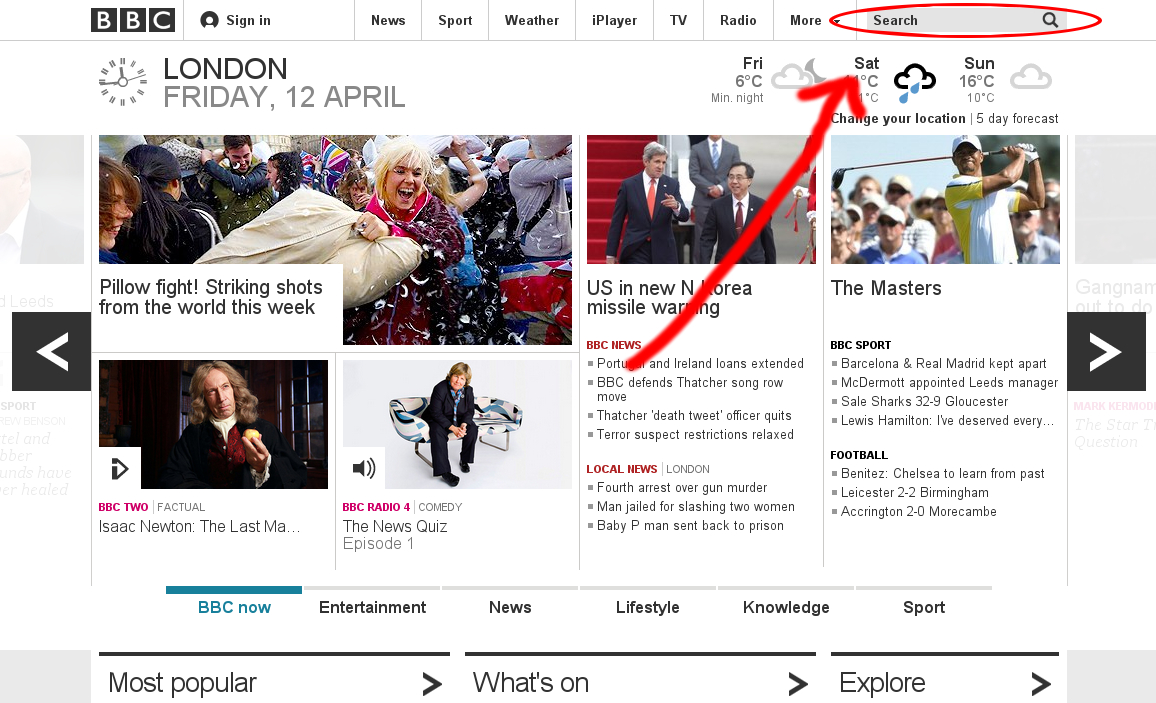
\includegraphics[width=\linewidth]{homepage.png}
\end{frame}
\note{
  I work in the team responsible for BBC's online search facility. The
  first point of entry is usually a the search box on the top right
  as shown. This then takes you to a search results page.
}
\begin{frame}
  \frametitle{BBC Search results}
  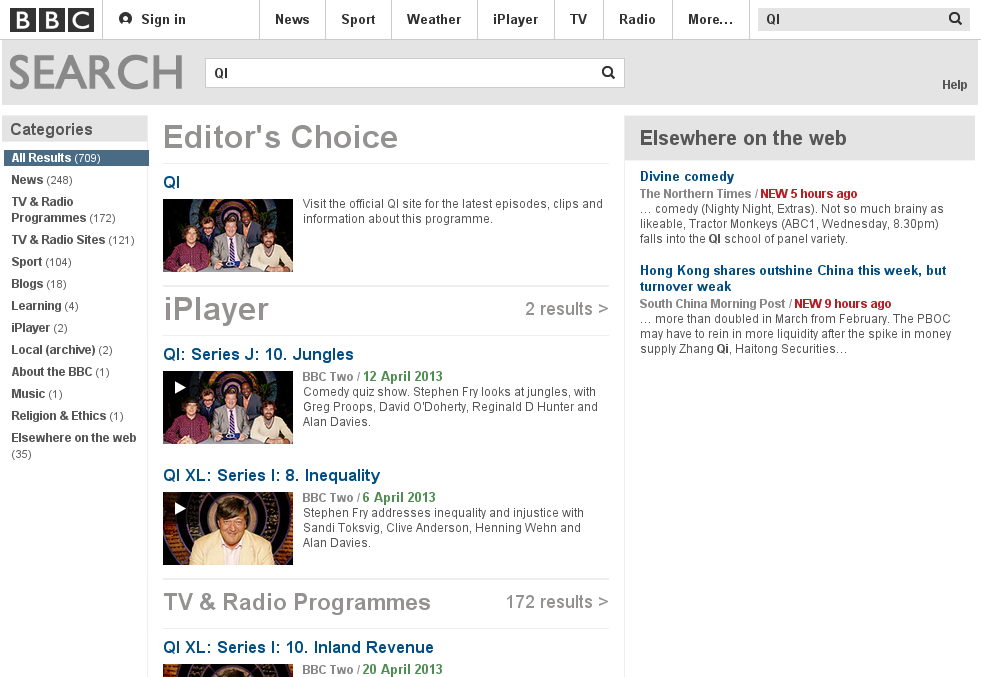
\includegraphics[width=\linewidth]{results.png}
\end{frame}
\note{
  This is the page you get after having done a search if you started
  on the home page as shown previously. You can see the first
  results are chosen by editors as the best results you are likely
  looking for.
}

\begin{frame}
  \frametitle{BBC iPlayer Search results}
  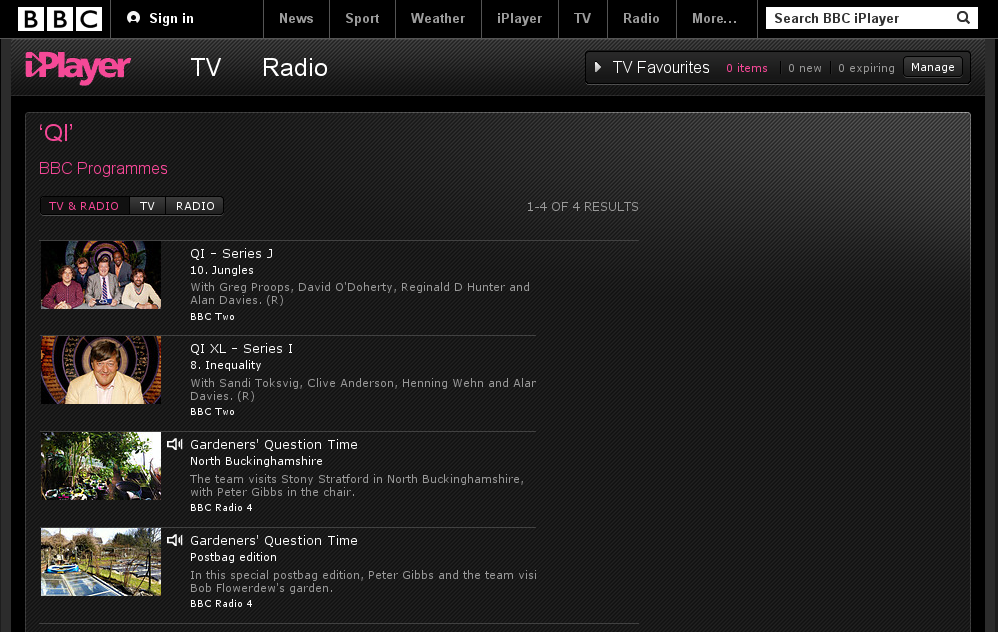
\includegraphics[width=\linewidth]{iplayer.png}
\end{frame}

\begin{frame}
  \frametitle{CBBC Search results}
  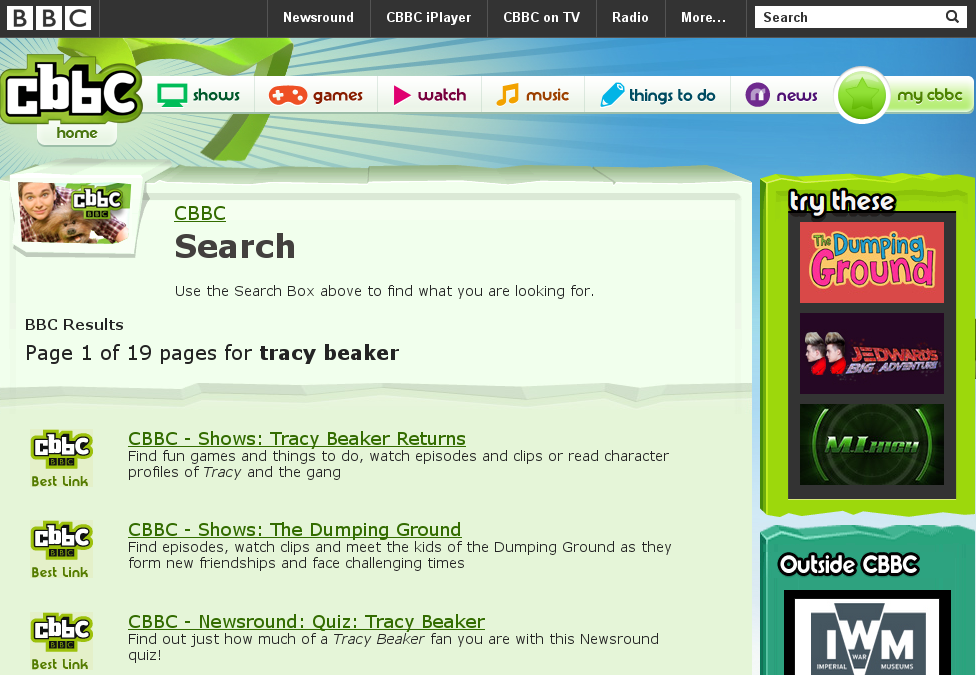
\includegraphics[width=\linewidth]{cbbc.png}
\end{frame}

\begin{frame}
  \frametitle{What's happening with BBC search?}
  \begin{itemize}
    \pause \item New team
    \begin{itemize}
    \pause \item Based in BBC North
    \end{itemize}
    \pause \item Improve architecture
    \pause \item Improve user experience
  \end{itemize}
\end{frame}

\begin{frame}
  \frametitle{Outline of this talk}
  \begin{enumerate}
    \pause \item What is web search?
    \pause \item Search techniques
    \pause \item Search design patterns
    \pause \item Why does BBC have its own search?
    \pause \item What does the BBC have online?
    \pause \item What does BBC Search look like as software system?
    \pause \item Model-View-Controller (MVC)
    \pause \item Service-Orientated Architecture (SOA)
    \pause \item Event-Driven Architecture (EDA)
    \pause \item How can we index BBC content?
    \pause \item How do we search BBC content?
    \pause \item How can we keep improving the experience?
  \end{enumerate}
\end{frame}

\begin{frame}[fragile]
  \frametitle{What is web search?}
  \begin{center}
    \begin{dot2tex}[dot,mathmode,scale=0.8]
      digraph G {
        rankdir=LR;
        node [shape="circle"];
        Crawling -> Indexing -> Querying;
      }
    \end{dot2tex}
  \end{center}
  \begin{enumerate}
    \item Crawl the web to find new pages
    \item Index pages to make it easier to search
    \item Searching/querying the page index
  \end{enumerate}
\end{frame}

\begin{frame}
  \frametitle{Web Crawlers}
  \begin{enumerate}
    \item Visit a page already known about
    \item Add that page to the search index
    \item Find all the links in that page
    \item Store all those links and visit them as well
  \end{enumerate}
\end{frame}

\begin{frame}
  \frametitle{Extracting Content}
  Crawlers/Spiders, Last-Modified, Extracting content
\end{frame}

\begin{frame}
  \frametitle{Indexing}
  \begin{itemize}
  \item Inverted Index
  \item Stemming? Tokenisation? Lemmatisation?
  \end{itemize}
\end{frame}

\begin{frame}
  \frametitle{Searching the index}
\end{frame}

\begin{frame}
  \frametitle{Scoring}
\end{frame}

\begin{frame}
  \frametitle{Google Pagerank}
\end{frame}

\begin{frame}
  \frametitle{Standard Search Interface}
\end{frame}

\begin{frame}
  \frametitle{Autocomplete}
\end{frame}

\begin{frame}
  \frametitle{Autosuggest}
\end{frame}

\begin{frame}
  \frametitle{Spell Check}
\end{frame}

\begin{frame}
  \frametitle{Facets}
\end{frame}

\begin{frame}
  \frametitle{Localisation}
\end{frame}

\begin{frame}
  \frametitle{Advanced Search}
\end{frame}

\begin{frame}
  \frametitle{Similar}
  \framesubtitle{``More like this''}
\end{frame}

\begin{frame}
  \frametitle{Why BBC Search?}
  \framesubtitle{Isn't Google good enough?}
\end{frame}

\begin{frame}
  \frametitle{Understanding BBC TV Programmes}
\end{frame}

\begin{frame}
  \frametitle{Understanding BBC Radio Programmes}
\end{frame}

\begin{frame}
  \frametitle{Linking News and other content by topic}
\end{frame}

\begin{frame}
  \frametitle{Connecting iPlayer with Learning}
\end{frame}

\begin{frame}
  \frametitle{Presenting regional and local information}
\end{frame}

\begin{frame}
  \frametitle{Supporting domestic languages}
\end{frame}

\begin{frame}
  \frametitle{What does BBC Search look like?}
  High-level diagram
\end{frame}

\begin{frame}
  \frametitle{Model-View-Controller (MVC)}
\end{frame}

\begin{frame}
  \frametitle{The problem of too many (or too few) databases}
  Too many databases, single point of failure with one database (decoupling)
\end{frame}

\begin{frame}
  \frametitle{``Service Layer''}
  \framesubtitle{Decouples the web application from the database}
  Decoupling, no need for database
\end{frame}

\begin{frame}
  \frametitle{Providing APIs for other service and applications}
  \framesubtitle{Application Programming Interface}
\end{frame}

\begin{frame}
  \frametitle{Service Orientated Architecture}
  \framesubtitle{Modularity and distributed computing}
\end{frame}

\begin{frame}
  \frametitle{Problems when service interfaces change}
\end{frame}

\begin{frame}
  \frametitle{Information feeds have to be polled}
  \framesubtitle{Or the information producer needs a list of consumers to notify}
\end{frame}

\begin{frame}
  \frametitle{Events}
\end{frame}

\begin{frame}
  \frametitle{Event-Driven Architecture}
\end{frame}

\begin{frame}
  \frametitle{What does BBC Search service layer look like?}
\end{frame}

\begin{frame}
  \frametitle{Different data stores or Content Management Systems (CMS)}
\end{frame}

\begin{frame}
  \frametitle{Indexing programmes information}
  \framesubtitle{Structured data}
\end{frame}

\begin{frame}
  \frametitle{How do we know if a programme is available on iPlayer?}
  \framesubtitle{7-day window}
\end{frame}

\begin{frame}
  \frametitle{Indexing News and Sport stories}
  \framesubtitle{Rapidly-published, text content}
\end{frame}

\begin{frame}
  \frametitle{Indexing Children's games, Bitesize, etc.}
  \frametitle{Content vs. pages}
\end{frame}

\begin{frame}
  \frametitle{Web Crawling}
  \framesubtitle{Older pages, mothballed sites, etc.}
\end{frame}

\begin{frame}
  \frametitle{Items with no tags}
  \framesubtitle{Can we generate them?}
\end{frame}

\begin{frame}
  \frametitle{How do we search it all?}
\end{frame}

\begin{frame}
  \frametitle{Searching different types of content}
  \framesubtitle{Comparing apples and oranges}
\end{frame}

\begin{frame}
  \frametitle{Some things have lots of text}
  \framesubtitle{Some things have no text}
\end{frame}

\begin{frame}
  \frametitle{What categories and facets can we offer?}
\end{frame}

\begin{frame}
  \frametitle{How can we keep improving the experience?}
\end{frame}

\begin{frame}
  \frametitle{Analytics}
\end{frame}

\begin{frame}
  \frametitle{Popular searches}
\end{frame}

\begin{frame}
  \frametitle{TV/Radio Broadcasts}
\end{frame}

\begin{frame}
  \frametitle{Responding to major events}
  Riots, snow
\end{frame}

\begin{frame}
  \frametitle{``Obvious'' Ordering of things}
  Manchester United, Man City, Manchester
\end{frame}

\begin{frame}
  \frametitle{Awareness of time of day...}
  \framesubtitle{... or day of the week}
\end{frame}

\begin{frame}
  \frametitle{Location Awareness}
\end{frame}

\begin{frame}
  \frametitle{User Testing}
\end{frame}

\begin{frame}
  \frametitle{Social Media}
  Trends on Twitter, shares on Facebook
\end{frame}

\begin{frame}
  \frametitle{The Future}
  Solve all the problems raised
\end{frame}

\end{document}
